\documentclass[xcolor=table, 10pt, aspectratio=43]{beamer}
% !TEX engine = xelatex
%\usepackage{arev}
\usepackage{amsmath,amssymb,amscd}
\usepackage{dsfont}
\usepackage{mathrsfs}
\usepackage{yfonts}
\usepackage{bm}
\usepackage{graphicx}
\usepackage{tabularx}
\usepackage{animate}
\usepackage{pifont}
%\usepackage{ifthen}

\usepackage{xeCJK}
\usepackage{fontspec}
\newfontfamily\cjkfont{PingFang SC}
\setCJKmainfont{PingFang SC}
\newcolumntype{x}{>{\centering\arraybackslash}X}
\renewcommand{\arraystretch}{1.5}

\usepackage{tikz}
	\usetikzlibrary{calc}
	\usetikzlibrary{arrows,shapes, positioning, matrix}
	\usetikzlibrary{decorations.markings}
	\tikzstyle arrowstyle=[scale=1]
	\tikzstyle directed=[postaction={decorate,decoration={markings,
 	   mark=at position .15 with {\arrow[arrowstyle]{stealth}}}}]
\tikzstyle string=[thick,postaction={decorate,decoration={markings,
    mark=at position .55 with {\arrow[arrowstyle]{stealth}}}}]
\tikzstyle dual_string=[dashed,postaction={decorate,decoration={markings,
    mark=at position .55 with {\arrow[arrowstyle]{stealth}}}}]

\tikzstyle dw=[thick,postaction={decorate,decoration={markings,
    mark=at position 1 with {\arrow[arrowstyle]{stealth}}}}]
\tikzstyle group=[mbg]

\usepackage{pgffor}
\newcommand{\mb}[1]{\mathbf{#1}}
\renewcommand{\cal}[1]{\mathcal{#1}}

\newcommand{\ag}[2]{#1_\mb{#2}}
\newcommand{\cohosub}[1]{\scalebox{0.72}{\textswab{#1}}}
\newcommand{\cohosubsub}[1]{\scalebox{0.6}{\textswab{#1}}}
\newcommand{\coho}[1]{\textswab{#1}}


\mode<presentation>
{
  %\usetheme{Warsaw}
  % or ...
  %\useoutertheme{rectangle}
  \setbeamertemplate{frametitle}[default][center]
  \defbeamertemplate{itemize item}{flat}{\begin{pgfpicture}{-1ex}{0ex}{1ex}{2ex}
      \pgfpathcircle{\pgfpoint{0pt}{.6ex}}{0.6ex}
      \pgfusepath{fill}
    \end{pgfpicture}%
  }
  \defbeamertemplate{itemize subitem}{flat}{\footnotesize\raise0.5pt\hbox{\textbullet}}
  \defbeamertemplate{itemize subsubitem}{flat}{\footnotesize\raise0.5pt\hbox{\textbullet}}

  %\useinnertheme{circles}
  \setbeamertemplate{items}[flat]
  \setbeamertemplate{sections/subsections in toc}[circle]
  \setbeamertemplate{blocks}[rounded]
  \setbeamertemplate{title page}[default][colsep=-4bp,rounded=true]
  \setbeamertemplate{part page}[default][colsep=-4bp,rounded=true]
  \setbeamercovered{transparent}
  %\usecolortheme{spruce}
  %\definecolor{THU}{RGB}{116,61,130}
  \definecolor{mbg}{RGB}{0,0,160}
  \setbeamercolor*{palette primary}{fg=white,bg=mbg}
  \setbeamercolor*{titlelike}{parent=palette primary}
  \setbeamercolor*{structure}{fg=mbg}
  \setbeamercolor{frametitle}{fg=white,bg=mbg}
  % or whatever (possibly just delete it)
  \setbeamercolor{block title}{bg=mbg,fg=white}
  \setbeamercolor{block body}{bg=mbg!15}


  \addtobeamertemplate{navigation symbols}{}{ \hspace{1em}%
    \usebeamerfont{footline}%
    \insertframenumber / \inserttotalframenumber }
}


%\usepackage[english]{babel}
% or whatever

%\usepackage[latin1]{inputenc}
% or whatever

%\usepackage{times}
%\usepackage[T1]{fontenc}
% Or whatever. Note that the encoding and the font should match. If T1
% does not look nice, try deleting the line with the fontenc.

\title[EQMC] % (optional, use only with long paper titles)
{Metals' awkward cousin is found}

\author[Y Qi] % (optional, use only with lots of authors)
{Yang~Qi}
% - Give the names in the same order as the appear in the paper.
% - Use the \inst{?} command only if the authors have different
%   affiliation.

\institute[Fudan] % (optional, but mostly needed)
{
Department of Physics, Fudan University.
}
% - Use the \inst command only if there are several affiliations.
% - Keep it simple, no one is interested in your street address.

%\date{2016 Annual Meeting of Fudan CFTPP} % (optional, should be abbreviation of conference name)
%{Fudan University, Oct 13 2015}
\date{Hefei, Oct 24, 2020.}
% - Either use conference name or its abbreviation.
% - Not really informative to the audience, more for people (including
%   yourself) who are reading the slides online

\subject{Theoretical Physics}
% This is only inserted into the PDF information catalog. Can be left
% out.



% If you have a file called "university-logo-filename.xxx", where xxx
% is a graphic format that can be processed by latex or pdflatex,
% resp., then you can add a logo as follows:

\pgfdeclareimage[height=1cm]{university-logo}{../resources/fudan}
\logo{\pgfuseimage{university-logo}}



% Delete this, if you do not want the table of contents to pop up at
% the beginning of each subsection:
\AtBeginSection[]
{
  \begin{frame}<beamer>{Outline}
			\tableofcontents[currentsection,currentsubsection]
  \end{frame}
}
%\AtBeginSubsection[]
%{
 % \begin{frame}<beamer>{Outline}
  %  \tableofcontents[currentsection,currentsubsection]
  %\end{frame}
%}


\begin{document}

\begin{frame}
  \titlepage
\end{frame}

\begin{frame}{Collaborators}
\begin{itemize}
\item Chuang Chen (陈闯), Institute of Physics, CAS.
\item Tian Yuan (袁天), Fudan University.
\item Xiao Yan Xu (许霄琰), UC San Diego.
\item Zi Yang Meng (孟子杨), Hong Kong University.
\begin{center}
  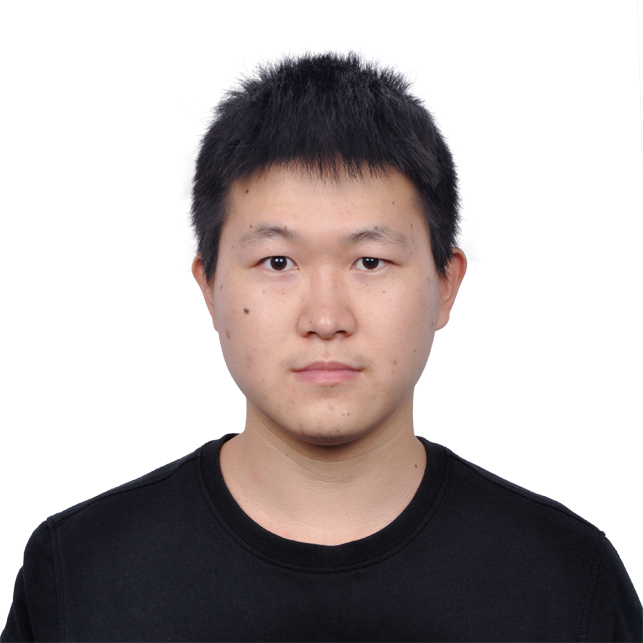
\includegraphics[height=2cm]{../people/chuangchen}
  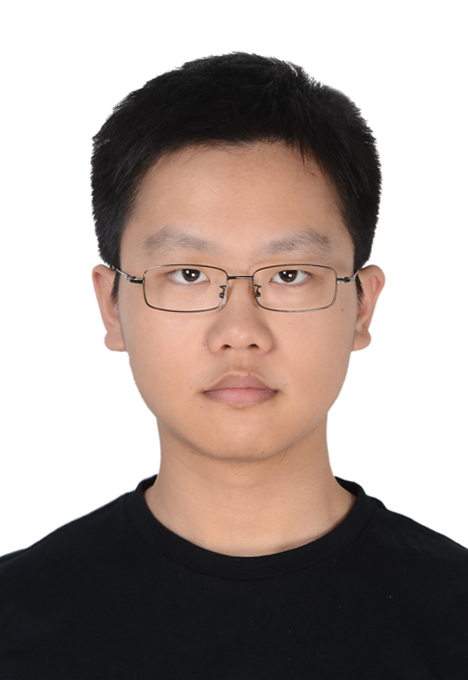
\includegraphics[height=2cm]{../people/tianyuan}
  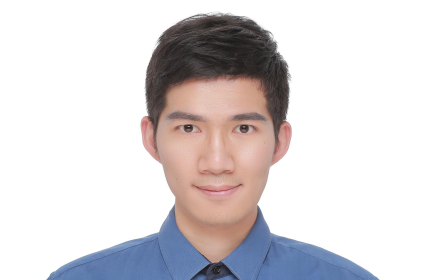
\includegraphics[height=2cm]{../people/xiaoyanxu}
  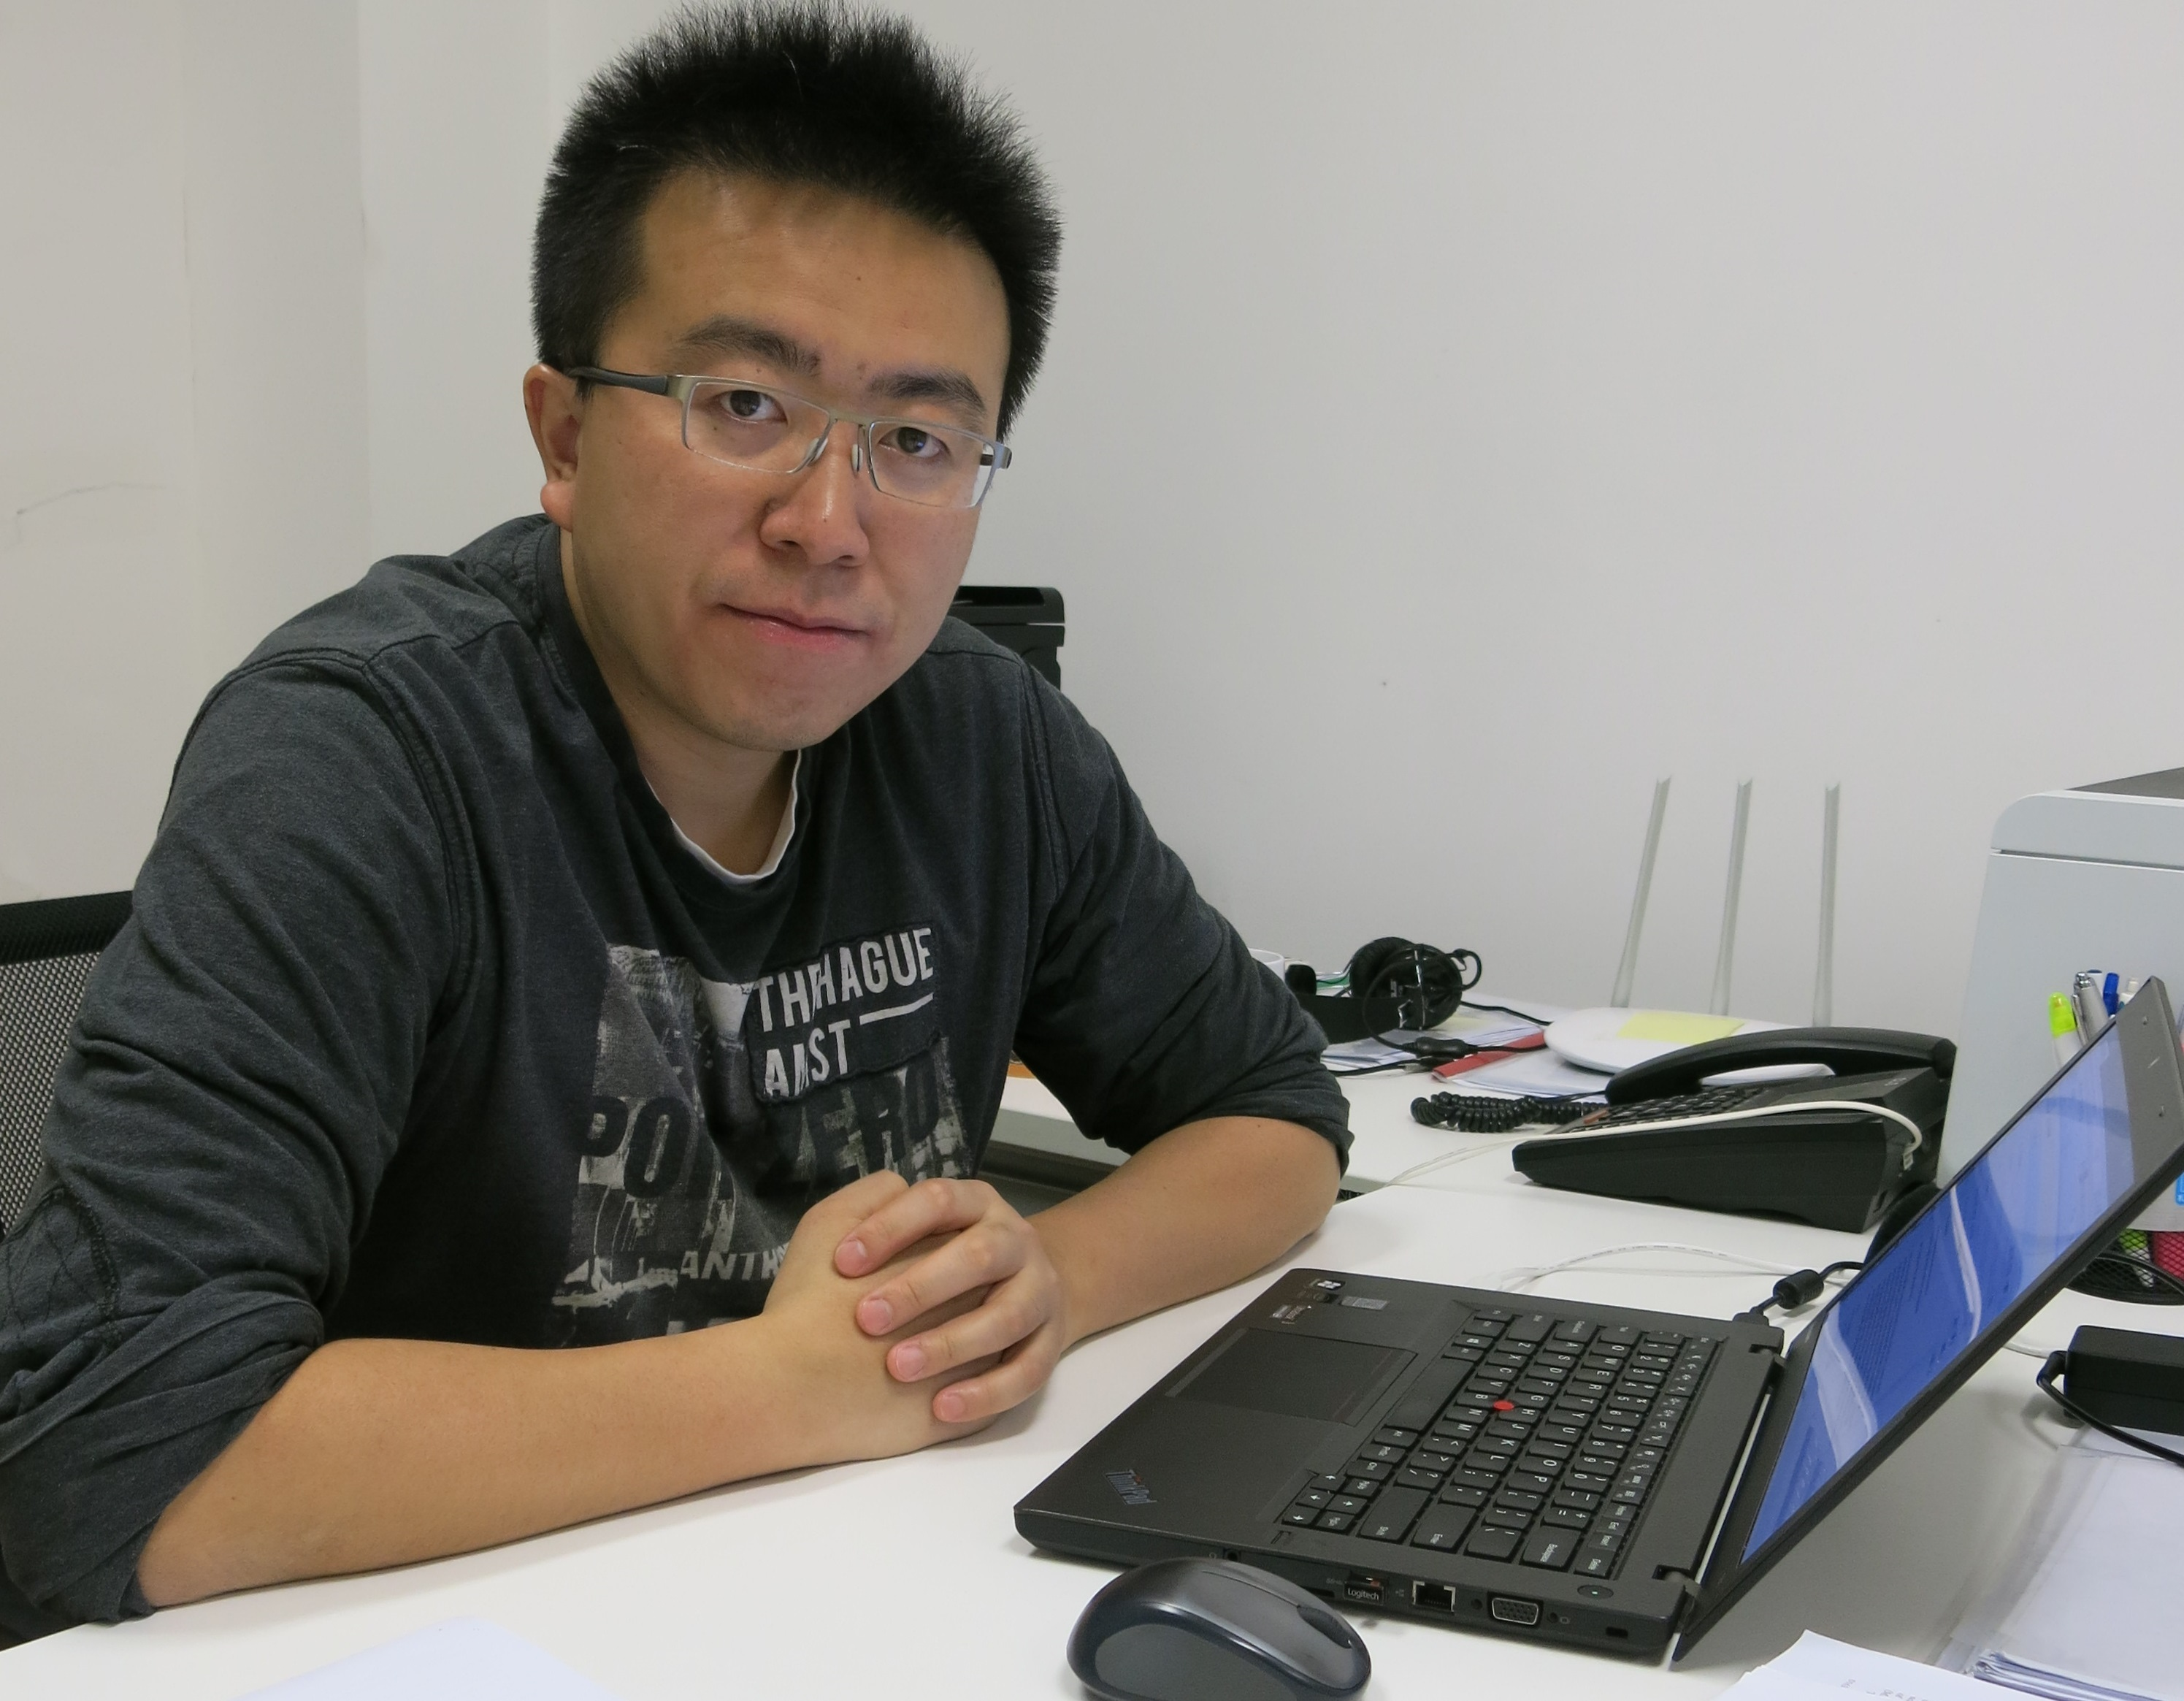
\includegraphics[height=2cm]{../people/ziyangmeng}
\end{center}
\end{itemize}
\begin{center}
  \small arXiv:2007.05543
\end{center}
\end{frame}

\begin{frame}{Outline}
	%\begin{columns}
	%\column{.7\textwidth}
		\tableofcontents
  %\end{columns}
  % You might wish to add the option [pausesections]
\end{frame}

\section{Introduction}

\begin{frame}
  \frametitle{Metal: Fermi surface}
\begin{itemize}
  \item Landau Fermi-Liquid Theory: a Fermi surface of quasiparticles.\\
  Noninteracting FS $\rightarrow$ Interacting FS.
  \item Volumn of the FS is conserved: Luttinger Thm.
\end{itemize}
\begin{center}
	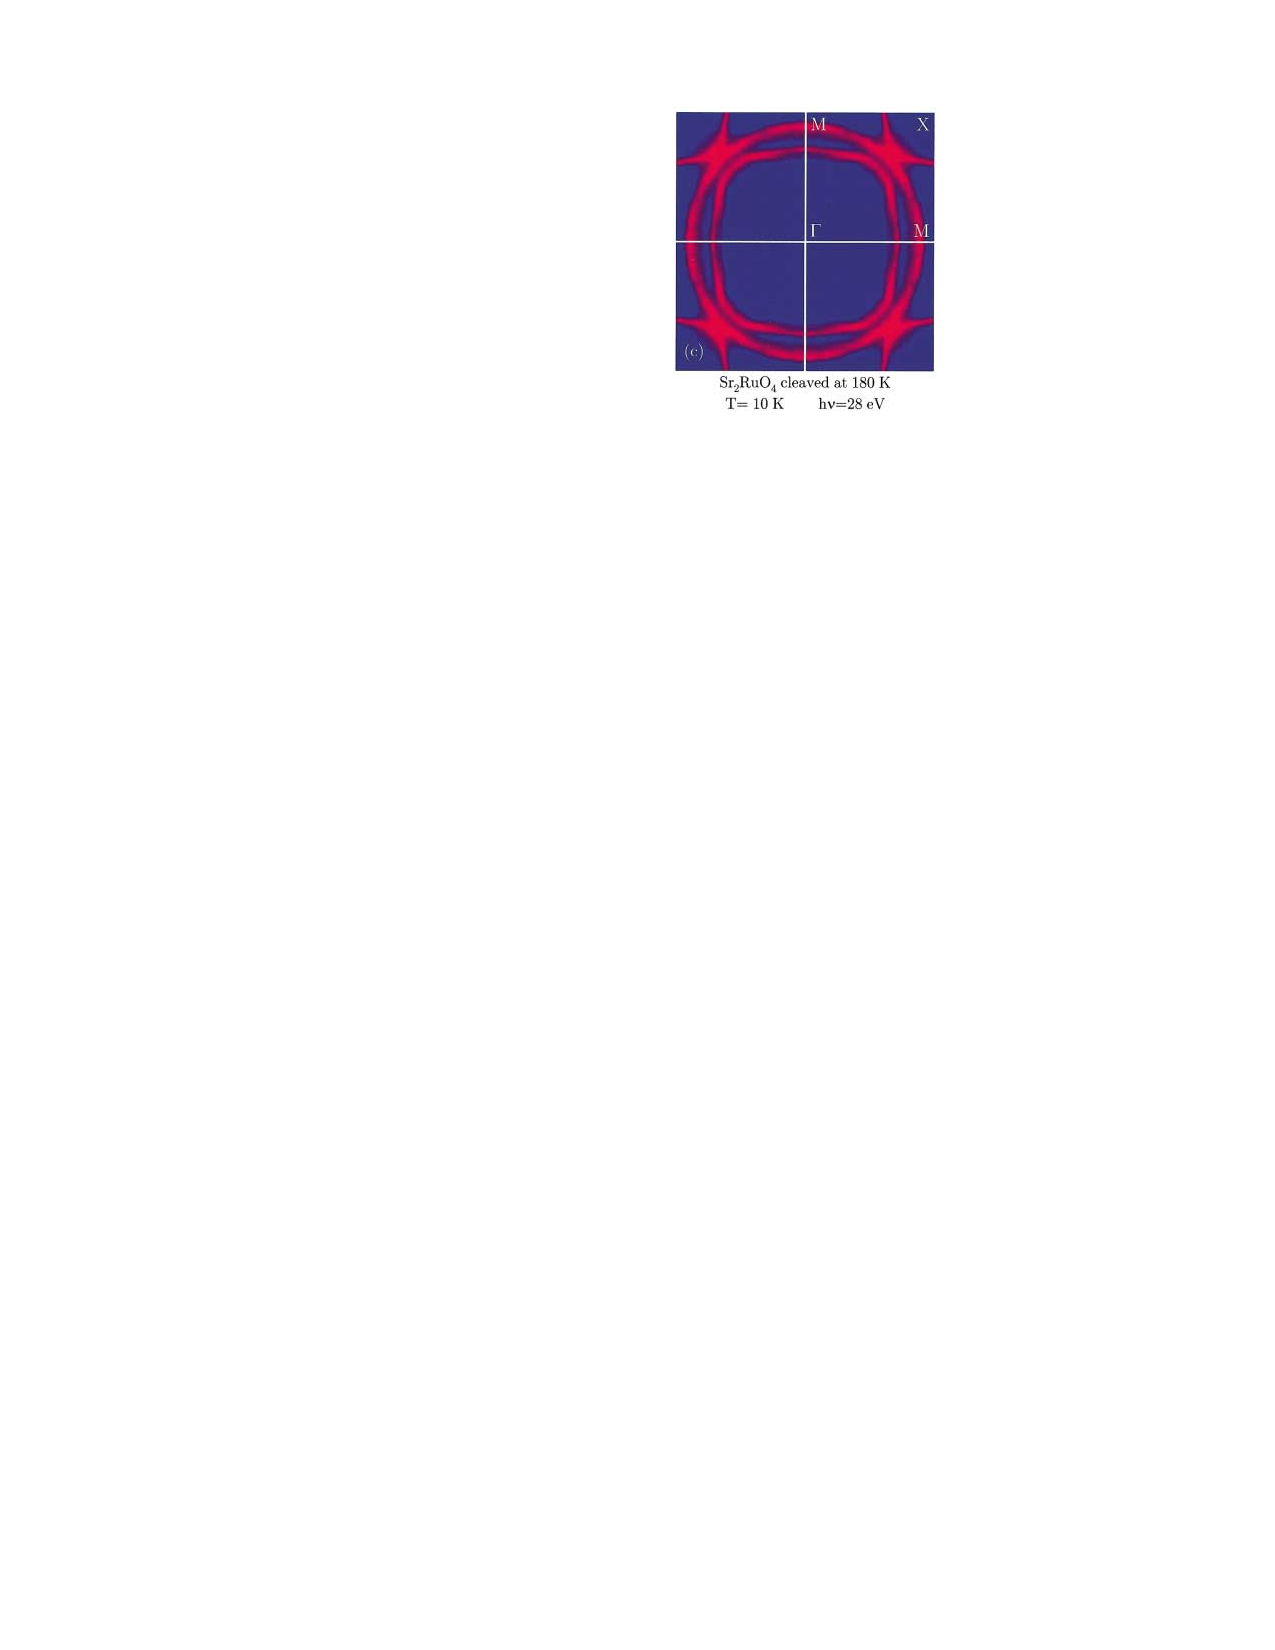
\includegraphics{../resources/SrRuO_FS}

	{\small A. Damascelli et al, PRL \textbf{85} 5194 (2000).}
\end{center}
\end{frame}

\begin{frame}
	\frametitle{Fermi arcs in high-Tc cuprates}
	\begin{columns}
		\column{.3\textwidth}
		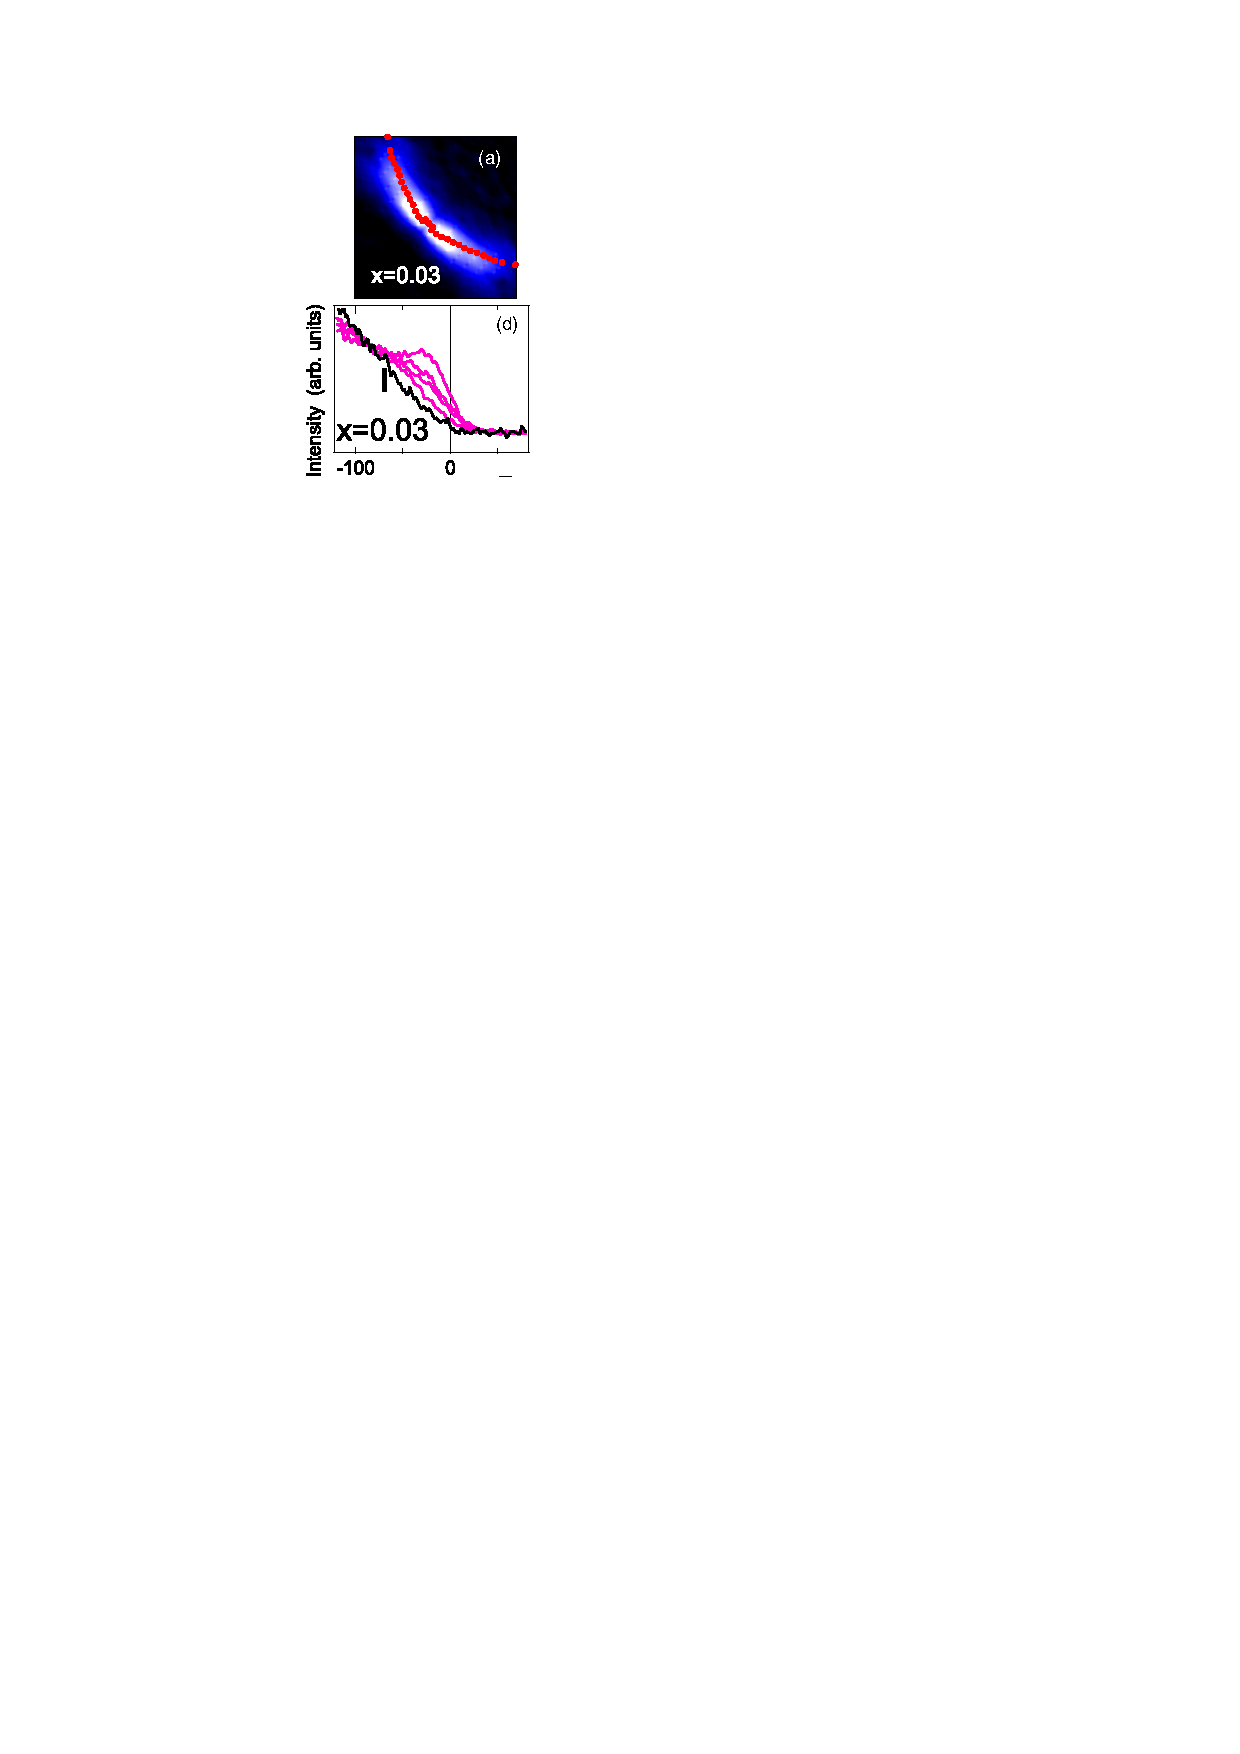
\includegraphics{arc_arpes}
		\column{.7\textwidth}
		\begin{itemize}
			\item Fermi arcs in underdoped cuprates: at $T_c<T<T^*$.
			\vspace{3em}
			\item A possible mechanism:
			$c_{i\sigma} = h_i^\dagger f_{i\sigma}$
			\item No satisfying theory.
		\end{itemize}
	\end{columns}
\end{frame}

\section{Model}

\begin{frame}
	\frametitle{The Model}
\begin{itemize}
\item Hamiltonian:
	\begin{align*}
	H_f &= -t\sum_{\langle i,j \rangle} (f^{\dagger}_{i,\alpha} \sigma^{z}_{b_{\langle i,j \rangle}}f_{j,\alpha} + h.c.) -\mu\sum_{i}f^{\dagger}_{i,\alpha}f_{i,\alpha}, \nonumber\\
	H_{z} &= -J \sum_{\langle i,j \rangle} S^{z}_{i} \sigma^{z}_{b_{\langle i,j \rangle}} S^{z}_{j} - h \sum_{i} S^{x}_{i}, \nonumber\\
	H_{g} &= -K \sum_{\square}\prod_{b\in\square} \sigma^{z}_{b} - g\sum_{b} \sigma^{x}_{b}.\\
	H_{c} &= -t \sum_{\langle i,j\rangle} f^{\dagger}_{i,\alpha}S^{z}_{i}f_{j,\alpha}S^{z}_{j} + h.c.
\end{align*}
\item Physical fermion $c_{i\alpha} = f_{i\alpha}S_i^z$
\end{itemize}
\begin{center}
	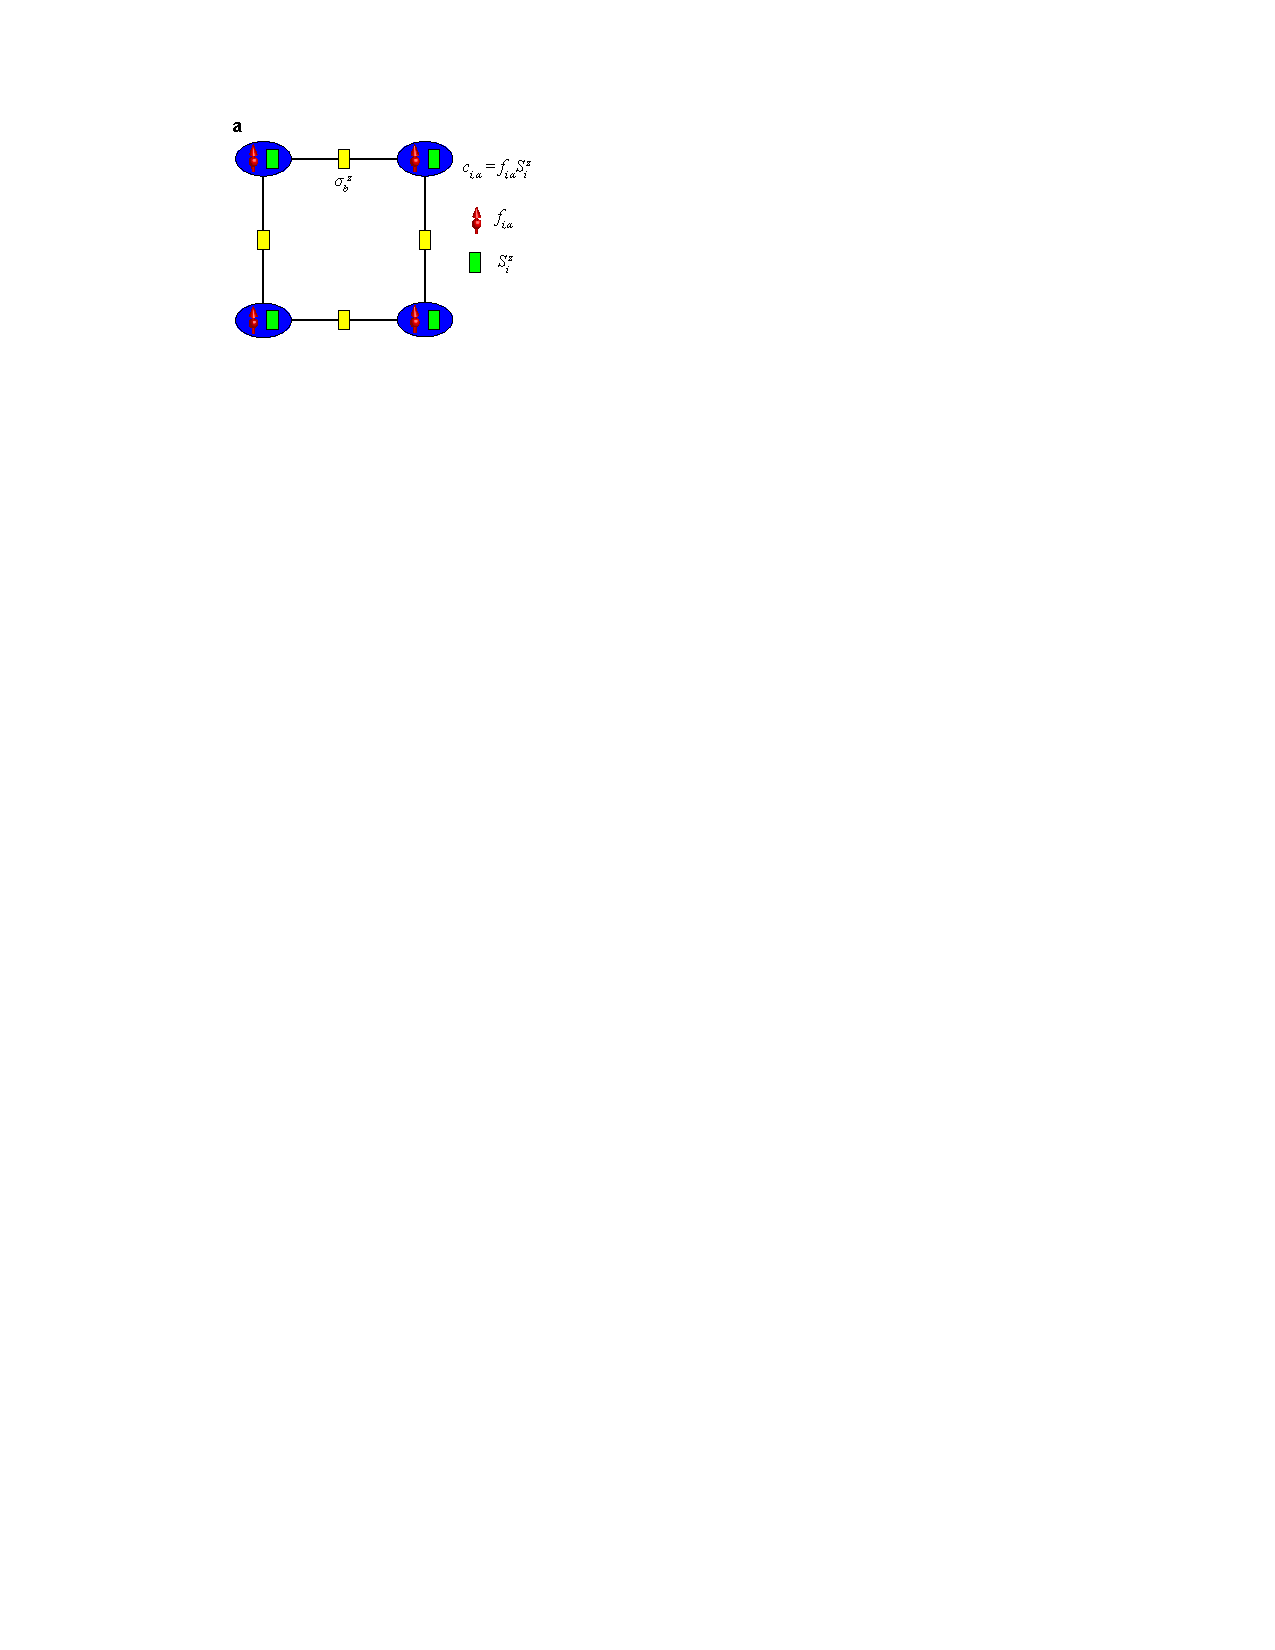
\includegraphics[width=4cm]{model_l}
\end{center}
\end{frame}

\begin{frame}
	\frametitle{The phase diagram}
	\begin{itemize}
		\item ``Fermi arc''
		\begin{itemize}
			\item[Ground state] Doped orthoginal metal.\\
			$f$-fermion fermi surface + gapped $S^z$ excitations.
			\item[Finite T] Fermi arcs.
		\end{itemize}
		\item Deconfined FL: $c$-fermion fermi surface + $\mathbb Z_2$ topological order.
		\item Confined FL: $c$-fermion fermi surface.
	\end{itemize}
	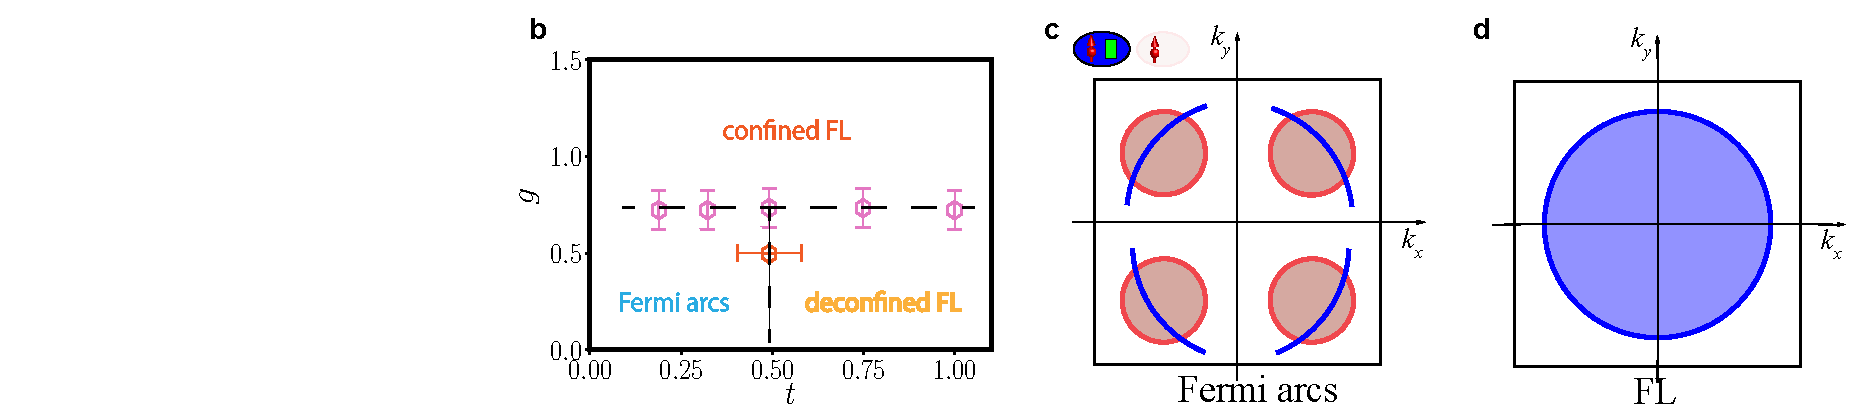
\includegraphics[width=\textwidth]{doped_pd}
\end{frame}

\section{DQMC simulation}

\begin{frame}
	\frametitle{Fermi arc}
	\begin{itemize}
		\item[(a)] Arc at finite $T$.
		\item[(b)] Spin susceptibility reveals hidden $f$-FS.
	\end{itemize}
	\begin{center}
		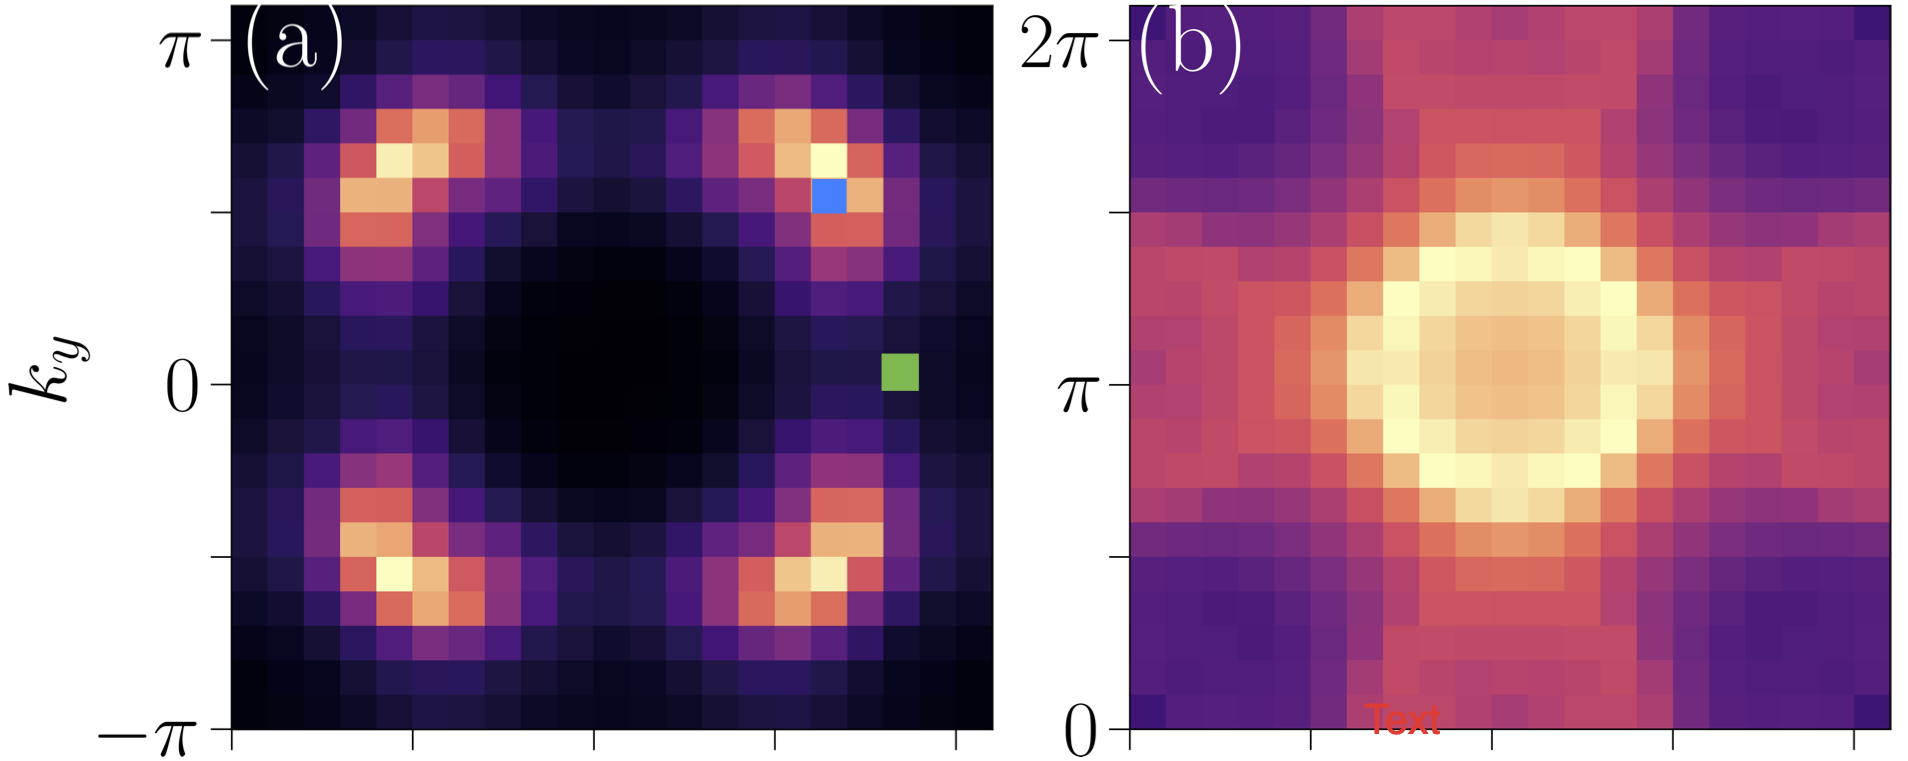
\includegraphics[height=3.5cm]{fermi_arc}\\
		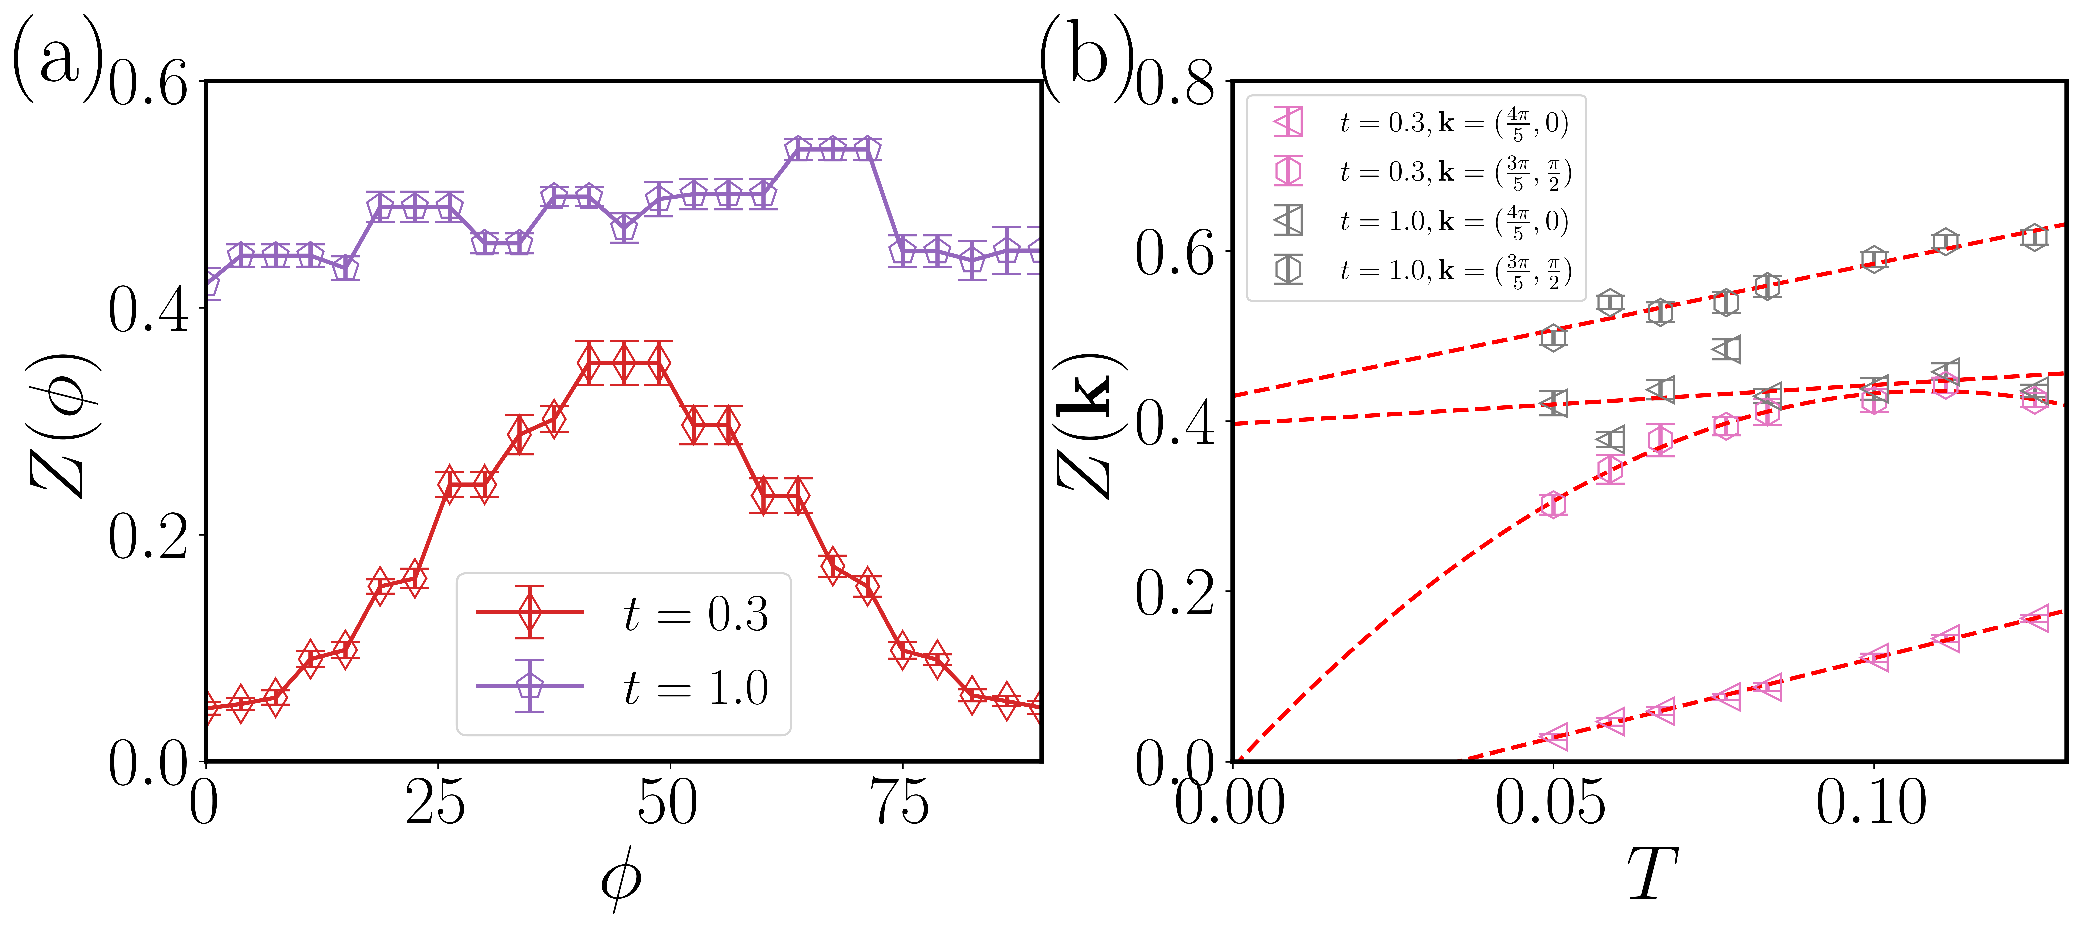
\includegraphics[height=3cm]{arc_T}
	\end{center}
\end{frame}

\begin{frame}
	\frametitle{Mean-field calculation}
	\begin{center}
		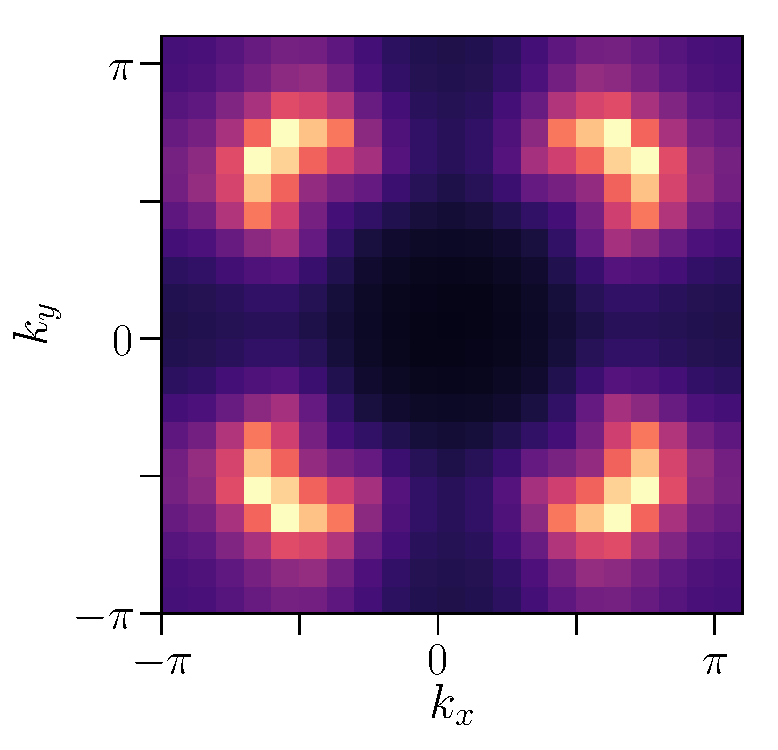
\includegraphics[height=4cm]{arc_mf}
	\end{center}
\end{frame}

\end{document}
